\DiaryEntry{Rational Points on the Unit Circle}{2016-06-23}{Maths}

Taken from ``Elliptic Tales: Curve Counting and Number Theory''.

\subsection{Unit Circle}

We have the unit circle given by points \((x,y)\) which are solution to

\[
x^2 + y^2 = 1
\]

There are four integer solutions \((1,0), (0,1), (-1,0), (0,-1)\).

\subsection{Rational Solutions}

We are interested in rational solutions; i.e. \(x, y \in \mathbb{Q}\).
We will show: If a line with rational slope which intersects the circle
at two points \(Q = (q_x, q_y), R = (r_x, r_y)\) and one of these points
has rational coordinates, then the other point also has rational
coordinates.

The line has the following equation: \(y = mx + b\) with \(m\) being
rational. If it intersects the circle at \(Q = (q_x, q_y)\) and
\(q_x, q_y\) are rational, we have \(q_y = m x + b\). Therefore,
\(b = q_y - m q_x\) and with \(q_y, m, q_x\) being rational, \(b\) will
also be rational.

If we insert the line equation into the circle equation, we obtain

\[
x^2 + (m x + b)^2 = 1
\]

which we can rewrite as

\[
(m^2 + 1) x^2 + (2mb)x + (b^2 - 1) = 0
\]

and refactor according to

\[
(m^2 + 1)(x - \alpha)(x - \beta) = 0
\]

where \(\alpha, \beta\) are the two roots of the quadratic polynomial.
We can further rewrite the expression as

\[
(m^2 + 1)\left( x^2 + (- \alpha - \beta) x  + \alpha \beta \right) = 0
\]

From this we can deduce that

\[
- (m^2 + 1) (\alpha +  \beta) = 2mb \rightarrow \alpha + \beta = -\frac{2mb}{m^2 + 1}
\]

Before we stated that \(m, b\) are rational numbers; therefore the
expression \(\alpha + \beta\) is also rational. Above we stated
\(Q = (q_x, q_y)\) intersects the circle - so one of the two roots
\(\alpha, \beta\) must equal \(q_x\). Without loss of generality, assume
this to be \(\alpha\): So \(q_x = \alpha\) and we have \(q_x + \beta\)
being something rational. From this it follows that \(\beta\) is also
rational. But \(\beta\) is the x-coordinate of \(R\), so we have
\(r_x = \beta\). Since \(R\) is also on the line, we have
\(r_y = m r_x + b = m \beta + b\). With \(m, \beta, b\) all being
rational, \(r_y\) is also rational and therefore \(R=(r_x, r_y)\) is a
rational point.

\subsection{Simplification}

By choosing one of the points cleverly, we can simplify things a bit: We
choose the point \(R=(r_x, r_y)\) as \(R=(-1,0)\): \(R\) has rational
coordinates and is also on the unit circle. Then the equation for the
line becomes \(y = mx+m\) and \(\beta=-1\). We know that

\[
q_x + \beta = -\frac{2mb}{m^2 + 1}
\]

and therefore \(q_x = \frac{1-m^2}{1+m^2}\). Using the line equation, we
obtain \(q_y = \frac{2m}{1+m^2}\).

The figure below shows the geometry involved. The line goes through the
point \(P=(0,m)\); if \(m\) is rational, then \(Q\) will have rational
coordinates given by the equations above.

\begin{figure}
\centering
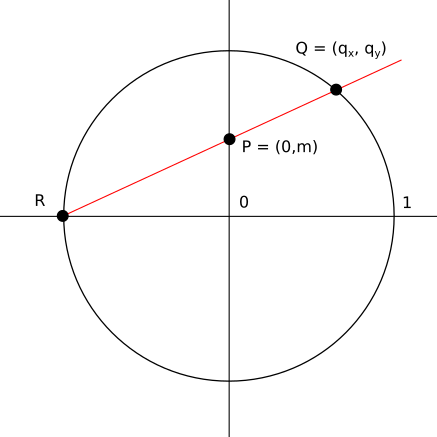
\includegraphics[scale=0.5]{images/rational_point_circle_01.png}
\end{figure}

\subsection{Interpretation}

The key point in the whole derivation is that there is a condition that
the sum of the roots, \(\alpha + \beta\), is rational. Now with the
condition that one root is rational, it follows that the other root is
also rational. If we would not consider a circle (a curve described by
an equation with degree 2), but a curve described by an equation of
higher order, this argument would no longer hold.
